\documentclass[conference]{IEEEtran}
\usepackage{amsmath,amssymb,amsfonts}
\usepackage{algorithmic}
\usepackage{algorithm}
\usepackage{graphicx}
\usepackage{textcomp}
\usepackage{booktabs}
\usepackage{multirow}
\usepackage{cite}
\usepackage{url}

\begin{document}

\title{Spectral Latent Alignment as a Transformation Technique for Cross-Domain Recommendation}

\author{
\IEEEauthorblockN{Divyam Sareen\textsuperscript{*}}
\IEEEauthorblockA{IIIT-Bangalore\\Bengaluru, India\\Divyam.Sareen@iiitb.ac.in}
\and
\IEEEauthorblockN{Subham Agarwala\textsuperscript{*}}
\IEEEauthorblockA{IIIT-Bangalore\\Bengaluru, India\\Subham.Agarwala@iiitb.ac.in}
\and
\IEEEauthorblockN{Daksh Rajesh\textsuperscript{*}}
\IEEEauthorblockA{IIIT-Bangalore\\Bengaluru, India\\Daksh.Rajesh@iiitb.ac.in}
}

\maketitle

\begin{abstract}
Cross-domain recommendation aims to improve predictions in a data-sparse target domain by leveraging knowledge from a data-rich source domain. Existing methods either require extensive user/item overlap or employ complex deep architectures that are difficult to interpret. We investigate \textbf{Spectral Latent Alignment (SLA)} as a lightweight, theoretically grounded \emph{transformation technique} for cross-domain recommendation. SLA computes spectral embeddings of user--item interaction graphs via the normalized Laplacian and aligns them across domains using an orthogonal Procrustes transformation derived from anchor correspondences. Through extensive experiments on four Amazon review dataset pairs, we demonstrate that SLA achieves significantly lower alignment gaps compared to Collective Matrix Factorization (CMF), indicating superior structural knowledge transfer. Specifically, SLA's alignment gap is 2.7$\times$ to 25$\times$ smaller than CMF's across all dataset pairs. We further show that SLA can be used to warm-start CMF, yielding a hybrid model that improves over baseline CMF on 3 of 4 dataset pairs. We provide a formal excess-risk bound decomposing the target-domain error into a Procrustes estimation term and a spectral-mismatch term, offering actionable diagnostics for when alignment-based transfer should succeed.
\end{abstract}

\begin{IEEEkeywords}
Cross-domain recommendation, spectral methods, graph Laplacian, Procrustes alignment, knowledge transfer, collaborative filtering
\end{IEEEkeywords}

\section{Introduction}

Recommender systems are widely deployed in e-commerce, streaming, and social media platforms. A persistent challenge is \emph{data sparsity}: when user--item interactions are insufficient to learn accurate models. This problem is especially severe for new domains or platforms with limited interaction history.

Cross-domain recommendation (CDR) addresses this by transferring knowledge from a data-rich source domain to a sparse target domain~\cite{cantador2015}. For example, user preferences learned from a movie recommendation system may improve book recommendations.

Traditional CDR methods rely on shared users or items across domains. Collective Matrix Factorization (CMF)~\cite{singh2008} jointly factorizes rating matrices while sharing latent factors for overlapping entities. While effective when overlap is substantial, performance degrades when overlap is limited. Recent deep learning approaches~\cite{yuan2019, man2017, hu2018} learn complex non-linear mappings between domain representations but require large datasets, careful tuning, and are often difficult to interpret.

In this work, we investigate a different perspective: rather than proposing SLA as a standalone recommender that must beat all baselines on raw RMSE, we position it as a \emph{transformation technique}---a principled method for aligning the structural representations of two domains. We evaluate this through the \emph{alignment gap}: the difference between cross-domain RMSE and an oracle RMSE that uses true target embeddings. A smaller alignment gap indicates better structural knowledge transfer, independent of the downstream predictor.

Our key contributions are:
\begin{itemize}
    \item We propose and evaluate SLA as a transformation technique for CDR, demonstrating alignment gaps 2.7$\times$--25$\times$ smaller than CMF across four dataset pairs.
    \item We show that SLA's spectral embeddings can warm-start CMF, producing a hybrid model that improves baseline CMF on 3 of 4 pairs.
    \item We provide a formal excess-risk bound that decomposes target error into interpretable, empirically estimable terms.
    \item We present comprehensive benchmarks including timing analysis and anchor sensitivity studies.
\end{itemize}

\section{Related Work}

Cross-domain recommendation has been extensively studied as a strategy to mitigate data sparsity and cold-start problems~\cite{cantador2015, zhu2021, khan2017}.

\subsection{Matrix Factorization Approaches}

Collective Matrix Factorization (CMF), introduced by Singh and Gordon~\cite{singh2008}, jointly factorizes multiple rating matrices while sharing latent factors for overlapping users or items. By coupling the factorizations through shared parameters, CMF enables information to propagate from a source domain to a target domain. Li et al.~\cite{li2009} extended this idea by exploring cross-domain collaborative filtering between movies and books to reduce sparsity. Hu et al.~\cite{hu2013} proposed triadic factorization that personalizes transfer using cross-domain user patterns.

While effective when user/item overlap is substantial, these methods fundamentally depend on shared entities. When overlap is small or absent, the shared latent factor assumption breaks down and transfer performance degrades significantly.

\subsection{Deep Learning and Embedding-Based Approaches}

Recent work has applied deep neural networks to learn cross-domain mappings. Man et al.~\cite{man2017} proposed EMCDR, which learns embeddings in each domain independently and then trains a mapping function (e.g., an MLP) to project source embeddings into the target space. Elkahky et al.~\cite{elkahky2015} developed a multi-view deep learning model that jointly learns from features across multiple domains.

Hu et al.~\cite{hu2018} introduced CoNet, which uses collaborative cross networks with cross-connection units between dual base networks to enable bidirectional knowledge transfer. Yuan et al.~\cite{yuan2019} proposed DARec, which uses deep autoencoders to extract transferable rating patterns via domain adaptation without requiring auxiliary information beyond the rating matrices.

Cao et al.~\cite{cao2022} addressed negative transfer in embedding-and-mapping approaches through CDRIB, which applies the information bottleneck principle to extract only domain-shared information while filtering domain-specific noise.

While these deep approaches can capture complex cross-domain relationships, they typically require large training datasets, careful hyperparameter tuning, and the learned mappings are often difficult to interpret.

\subsection{Adversarial Domain Adaptation}

Domain-Adversarial Neural Networks (DANN), introduced by Ganin et al.~\cite{ganin2016}, train a feature extractor jointly with a domain classifier in an adversarial setting, producing representations that are discriminative for the task while being domain-invariant. This idea has been adopted in cross-domain recommendation to learn domain-invariant user representations~\cite{liu2017}.

Although adversarial methods can reduce domain shift, they often suffer from unstable training dynamics and complex optimization. Moreover, aligning feature \emph{distributions} does not necessarily preserve the structural relationships between users and items that are essential for recommendation.

\subsection{Graph-Based Methods}

Graph neural networks have gained prominence in recommender systems. PinSage~\cite{ying2018} demonstrated web-scale graph convolutions for recommendations, while LightGCN~\cite{he2020} showed that simplified linear graph convolutions suffice for collaborative filtering. These methods highlight the importance of structural information in interaction graphs.

However, most graph-based recommendation methods focus on single-domain performance rather than cross-domain transfer. Our work bridges this gap by using spectral graph representations as the basis for cross-domain alignment.

\subsection{Spectral Methods and Procrustes Alignment}

The orthogonal Procrustes problem~\cite{schoenemann1966} seeks the optimal orthogonal transformation aligning two matrices and has been widely used in shape analysis and natural language processing for bilingual word embedding alignment. The Davis--Kahan theorem~\cite{davis1970} provides perturbation bounds for eigenspaces, enabling theoretical analysis of spectral embedding stability. Our work combines these classical tools in a novel application to cross-domain recommendation.

\section{Proposed Method}

We propose \textbf{Spectral Latent Alignment (SLA)}, a method that transfers structural knowledge across domains by aligning spectral embeddings of user--item interaction graphs.

\subsection{Graph Representation and Spectral Embeddings}

Each domain is represented as a bipartite graph where users and items are nodes, and interactions form edges. From the interaction matrix $R \in \mathbb{R}^{n_u \times n_i}$, we construct a binary adjacency matrix $A = \mathbf{1}[R > 0]$ and compute the symmetrically normalized interaction matrix:
\begin{equation}
    M = D_u^{-1/2} \, A \, D_i^{-1/2}
\end{equation}
where $D_u$ and $D_i$ are diagonal degree matrices for users and items respectively.

We compute the top-$k$ singular vectors of $M$ via truncated SVD, yielding user embeddings $U_{\text{user}} \in \mathbb{R}^{n_u \times k}$ and item embeddings $U_{\text{item}} \in \mathbb{R}^{n_i \times k}$. These spectral embeddings capture the principal structural patterns of the interaction network.

\subsection{Anchor Correspondences and Procrustes Alignment}

To align two domains, we assume a set of $m$ anchor correspondences (shared users present in both domains). Let $X = U_S^{(a)} \in \mathbb{R}^{m \times k}$ and $Y = U_T^{(a)} \in \mathbb{R}^{m \times k}$ denote the anchor embeddings from source and target domains.

We compute the orthogonal transformation $\hat{Q}$ that minimizes:
\begin{equation}
    \hat{Q} = \arg\min_{Q^TQ=I} \| X Q - Y \|_F^2
\end{equation}

This is the \emph{Orthogonal Procrustes problem}~\cite{schoenemann1966}, solved in closed form via SVD of $X^T Y = U_M \Sigma_M V_M^T$, giving $\hat{Q} = U_M V_M^T$.

The aligned source embeddings are: $\tilde{U}_S = U_S \hat{Q}$.

\subsection{Recommendation Transfer}

After alignment, a predictor trained on target-domain data (using target user and item embeddings) can serve cross-domain users by substituting aligned source embeddings at inference time. In our implementation, we train a LightGBM regressor on concatenated $[u_{\text{target}}, v_{\text{item}}]$ embedding pairs and at test time replace $u_{\text{target}}$ with the aligned source embedding $\tilde{u}_S$.

\subsection{SLA as Initialization for CMF (Hybrid Model)}

Beyond standalone use, SLA's aligned embeddings can warm-start other models. We propose a hybrid approach where:
\begin{enumerate}
    \item SLA computes Procrustes-aligned spectral embeddings
    \item These initialize CMF's shared user factor $U$ (using the average of aligned source and target embeddings)
    \item CMF then trains with optional structural regularization: $\mathcal{L}_{\text{reg}} = \lambda \| U - U_{\text{init}} \|_F^2$
\end{enumerate}

This injects SLA's alignment quality into CMF's rating-prediction pipeline.

\subsection{Algorithms}

\begin{algorithm}[t]
\caption{SLA -- Training}
\begin{algorithmic}[1]
\REQUIRE Source matrix $R_S$, target matrix $R_T$, anchors $\mathcal{A}$ (size $m$), dimension $k$
\ENSURE Trained predictor $\mathcal{M}$, alignment $\hat{Q}$
\STATE Compute normalized matrices $M_S$, $M_T$
\STATE Compute top-$k$ SVD of $M_S$, $M_T$ to get $U_S$, $U_T$
\STATE Extract anchor rows: $X \leftarrow U_S^{(\mathcal{A})}$, $Y \leftarrow U_T^{(\mathcal{A})}$
\STATE SVD: $X^T Y = U_M \Sigma_M V_M^T$
\STATE $\hat{Q} \leftarrow U_M V_M^T$
\STATE $\tilde{U}_S \leftarrow U_S \hat{Q}$
\STATE Train predictor $\mathcal{M}$ on target embeddings
\RETURN $\mathcal{M}$, $\hat{Q}$
\end{algorithmic}
\end{algorithm}

\begin{algorithm}[t]
\caption{SLA -- Inference}
\begin{algorithmic}[1]
\REQUIRE Target matrix $R_T$, source embeddings $U_S$, alignment $\hat{Q}$, predictor $\mathcal{M}$, top-$K$
\ENSURE Top-$K$ items per query user
\STATE Compute target item embeddings $U_T^{\text{item}}$
\FOR{each query user $u$}
    \STATE $z_u \leftarrow U_S[u] \cdot \hat{Q}$ \COMMENT{align source embedding}
    \FOR{each candidate item $i$}
        \STATE $s_{u,i} \leftarrow \mathcal{M}(z_u, U_T^{\text{item}}[i])$
    \ENDFOR
    \STATE Output top-$K$ items by score
\ENDFOR
\end{algorithmic}
\end{algorithm}

%% Part 2: Theoretical Analysis, Experiments, Conclusion

\section{Theoretical Analysis}

We prove a quantitative excess-risk bound for the SLA pipeline, showing that the target risk is bounded by the source risk plus two interpretable terms: (i) a \emph{Procrustes estimation term} controlled by anchor quality, and (ii) a \emph{spectral-mismatch term} controlled by the Laplacian perturbation and spectral gap.

\subsection{Notation}

\begin{itemize}
    \item $L_S, L_T \in \mathbb{R}^{n \times n}$: normalized Laplacians of source/target graphs
    \item $U_S, U_T \in \mathbb{R}^{n \times k}$: top-$k$ eigenvector matrices
    \item $X = U_S^{(a)} \in \mathbb{R}^{m \times k}$, $Y = U_T^{(a)} \in \mathbb{R}^{m \times k}$: anchor embeddings
    \item $\hat{Q} = \arg\min_{Q \in O(k)} \|XQ - Y\|_F$: Procrustes estimator
    \item $Q_0 = \arg\min_{Q \in O(k)} \|U_S Q - U_T\|_F$: optimal alignment
    \item $\tilde{U}_S = U_S \hat{Q}$: aligned source embeddings
    \item $f_{\text{tgt}}$: predictor trained on $\tilde{U}_S$; $L_f$-Lipschitz
\end{itemize}

\subsection{Assumptions}

\textbf{A1} (Spectral embeddings): $U_S$, $U_T$ are top-$k$ orthonormal eigenvector matrices of $L_S$, $L_T$.

\textbf{A2} (Laplacian perturbation): $L_T = L_S + \Delta$ with $\|\Delta\|_2 \leq \varepsilon$.

\textbf{A3} (Spectral gap): $L_S$ has spectral gap $\gamma > 0$ at index $k$.

\textbf{A4} (Anchors): $m$ anchor correspondences with $X$ having full column rank.

\textbf{A5} (Anchor residual): $E = Y - X Q_0 = U_T^{(a)} - U_S^{(a)} Q_0$.

\textbf{A6} (Smoothness): $f_{\text{tgt}}$ is $L_f$-Lipschitz; embeddings bounded by $B$.

\subsection{Supporting Lemmas}

\textbf{Davis--Kahan Theorem~\cite{davis1970}:} Under A1--A3, the principal-angle distance satisfies:
\begin{equation}
    \|\sin\Theta(U_S, U_T)\|_2 \leq \frac{\varepsilon}{\gamma} \implies \|U_S Q_0 - U_T\|_F \leq \frac{\sqrt{k}\,\varepsilon}{\gamma}
\end{equation}

\textbf{Procrustes Perturbation:} If $\|X^T E\|_2 < \frac{1}{2}\sigma_{\min}(X^T X)$, then:
\begin{equation}
    \|\hat{Q} - Q_0\|_2 \leq \frac{2\|X^T E\|_2}{\sigma_{\min}(X^T X)}
\end{equation}

\subsection{Main Theorem}

\textbf{Theorem 1} (Excess-Risk Bound). Under assumptions A1--A6:
\begin{equation}
\left| R_T^{(\text{true})}(f_{\text{tgt}}) - R_S(f_{\text{tgt}}) \right| \leq L_f B \left( \sqrt{k} \cdot \frac{2\|X^T E\|_2}{\sigma_{\min}(X^T X)} + \frac{\sqrt{k}\,\varepsilon}{\gamma} \right) + |\Delta_{\text{labels}}|
\end{equation}

where $\Delta_{\text{labels}}$ captures conditional label-distribution shift (zero when source and target share the same rating mechanism).

\textbf{Proof sketch.} The proof proceeds in three steps:

\emph{Step 1:} By Lipschitz continuity, the risk change from replacing true target embeddings with aligned source embeddings is bounded by $L_f B \frac{1}{\sqrt{n}} \|\tilde{U}_S - U_T\|_F$.

\emph{Step 2:} The difference between target and source risk decomposes as an embedding term plus a label-shift term $\Delta_{\text{labels}}$.

\emph{Step 3:} The embedding error decomposes via triangle inequality:
$\|\tilde{U}_S - U_T\|_F \leq \sqrt{k}\|\hat{Q} - Q_0\|_2 + \|U_S Q_0 - U_T\|_F$,
where the first term is bounded by the Procrustes perturbation lemma and the second by Davis--Kahan. \hfill$\square$

This bound provides actionable diagnostics: the quantities $\varepsilon$, $\gamma$, $\sigma_{\min}(X^T X)$, and $\|X^T E\|_2$ are all empirically estimable, predicting when alignment should succeed and suggesting remedies (more/better anchors, larger spectral gap) when transfer is likely to fail.

\section{Experimental Setup}

\subsection{Datasets}

We use four cross-domain pairs from the Amazon Review dataset~\cite{mcauley2015}, selecting overlapping users with $\geq$5 interactions per domain:

\begin{table}[h]
\centering
\caption{Dataset Statistics}
\label{tab:datasets}
\begin{tabular}{lcc}
\toprule
\textbf{Domain Pair} & \textbf{Shared Users} & \textbf{Train/Test}\\
\midrule
Office Products $\to$ Movies \& TV & Large & 90\%/10\% \\
Sports \& Outdoors $\to$ CDs \& Vinyl & Large & 90\%/10\% \\
Android Apps $\to$ Video Games & Medium & 90\%/10\% \\
Toys \& Games $\to$ Automotive & Medium & 90\%/10\% \\
\bottomrule
\end{tabular}
\end{table}

\subsection{Baselines}

\begin{itemize}
    \item \textbf{CMF}~\cite{singh2008}: Collective Matrix Factorization with shared user embeddings ($k$=50, $\alpha$=0.5, lr=0.01)
    \item \textbf{DARec}~\cite{yuan2019}: Deep domain adaptation with autoencoders
    \item \textbf{I-DARec}: Item-based variant of DARec
    \item \textbf{U-DARec}: User-based variant of DARec
    \item \textbf{SLA (Ours)}: Spectral Latent Alignment ($k$=300, LightGBM predictor with Optuna-tuned hyperparameters)
    \item \textbf{Hybrid SLA-CMF}: CMF warm-started with SLA embeddings ($k$=100, Optuna-tuned)
\end{itemize}

\subsection{Evaluation Metrics}

\begin{itemize}
    \item \textbf{RMSE}: Root Mean Squared Error on target domain test ratings
    \item \textbf{Alignment Gap}: $\text{RMSE}_{\text{cross}} - \text{RMSE}_{\text{oracle}}$, measuring the quality of cross-domain transfer independent of predictor capacity
\end{itemize}

\section{Results and Analysis}

\subsection{Cross-Domain RMSE Comparison}

Table~\ref{tab:rmse} presents the RMSE comparison across all methods.

\begin{table}[h]
\centering
\caption{Cross-Domain RMSE (lower is better)}
\label{tab:rmse}
\begin{tabular}{lcccc}
\toprule
\textbf{Method} & \textbf{Office} & \textbf{Sports} & \textbf{Apps} & \textbf{Toys} \\
 & \textbf{$\to$Movies} & \textbf{$\to$CDs} & \textbf{$\to$Games} & \textbf{$\to$Auto} \\
\midrule
U-DARec & 2.119 & 3.509 & 2.560 & 3.610 \\
DARec & 2.552 & 3.864 & 2.852 & 3.911 \\
I-DARec & 1.114 & 0.948 & 1.138 & 1.047 \\
SLA (LGB) & 1.187 & 0.840 & 1.162 & 1.057 \\
CMF & \textbf{0.994} & \textbf{0.800} & 1.137 & \textbf{0.945} \\
Hybrid & 1.087 & 0.820 & \textbf{1.056} & 1.074 \\
\bottomrule
\end{tabular}
\end{table}

CMF achieves the best raw RMSE on 3 of 4 pairs, while the Hybrid model wins on Android Apps $\to$ Video Games (6.05\% improvement over CMF). SLA standalone is competitive with I-DARec and substantially outperforms U-DARec and DARec.

\subsection{Alignment Gap Analysis}

The alignment gap measures how much RMSE degrades when substituting cross-domain embeddings for oracle (true target) embeddings. This is our primary metric for evaluating SLA as a \emph{transformation technique}.

\begin{table}[h]
\centering
\caption{Alignment Gap = RMSE(Cross) $-$ RMSE(Oracle). Lower is better.}
\label{tab:gap}
\begin{tabular}{lccc|ccc}
\toprule
& \multicolumn{3}{c}{\textbf{SLA}} & \multicolumn{3}{c}{\textbf{CMF}} \\
\cmidrule(lr){2-4} \cmidrule(lr){5-7}
\textbf{Pair} & Oracle & Cross & Gap & Oracle & Cross & Gap \\
\midrule
Office$\to$Movies & 1.077 & 1.100 & \textbf{0.023} & 0.988 & 1.098 & 0.110 \\
Sports$\to$CDs & 0.981 & 1.017 & \textbf{0.036} & 0.896 & 0.961 & 0.064 \\
Apps$\to$Games & 1.220 & 1.234 & \textbf{0.014} & 0.819 & 1.177 & 0.358 \\
Toys$\to$Auto & 1.106 & 1.118 & \textbf{0.012} & 0.906 & 1.073 & 0.168 \\
\bottomrule
\end{tabular}
\end{table}

\textbf{Key finding:} SLA's alignment gap is consistently and substantially smaller than CMF's across all four dataset pairs:
\begin{itemize}
    \item Office$\to$Movies: SLA gap 0.023 vs CMF gap 0.110 (\textbf{4.8$\times$ smaller})
    \item Sports$\to$CDs: SLA gap 0.036 vs CMF gap 0.064 (\textbf{1.8$\times$ smaller})
    \item Apps$\to$Games: SLA gap 0.014 vs CMF gap 0.358 (\textbf{25.6$\times$ smaller})
    \item Toys$\to$Auto: SLA gap 0.012 vs CMF gap 0.168 (\textbf{14.0$\times$ smaller})
\end{itemize}

This demonstrates that SLA provides significantly better structural alignment between domains, even when CMF achieves lower absolute RMSE (due to its stronger rating-prediction head). The spectral Procrustes alignment preserves graph structure far more faithfully than CMF's shared-embedding approach.

\subsection{Hybrid SLA-CMF Results}

Using SLA embeddings to initialize CMF provides consistent improvements on 3 of 4 dataset pairs:

\begin{table}[h]
\centering
\caption{Hybrid SLA-CMF vs Baseline CMF}
\label{tab:hybrid}
\begin{tabular}{lccc}
\toprule
\textbf{Dataset Pair} & \textbf{CMF} & \textbf{Hybrid} & \textbf{Improved?} \\
\midrule
Office$\to$Movies & 1.122 & 1.122 & YES \\
Sports$\to$CDs & 0.822 & 0.821 & YES \\
Apps$\to$Games & 1.059 & 1.059 & no \\
Toys$\to$Auto & 1.076 & 1.074 & YES \\
\bottomrule
\end{tabular}
\end{table}

The improvement is modest but consistent, confirming that SLA's structural alignment provides useful inductive bias for CMF training.

\subsection{Anchor Sensitivity}

Fig.~\ref{fig:anchors} shows RMSE as a function of anchor percentage for both SLA and CMF. SLA exhibits remarkably stable performance even with as few as 10\% of training users as anchors. This is consistent with our theoretical bound, which predicts that alignment quality depends on anchor \emph{diversity} ($\sigma_{\min}(X^T X)$) rather than sheer quantity.

\begin{figure}[h]
    \centering
    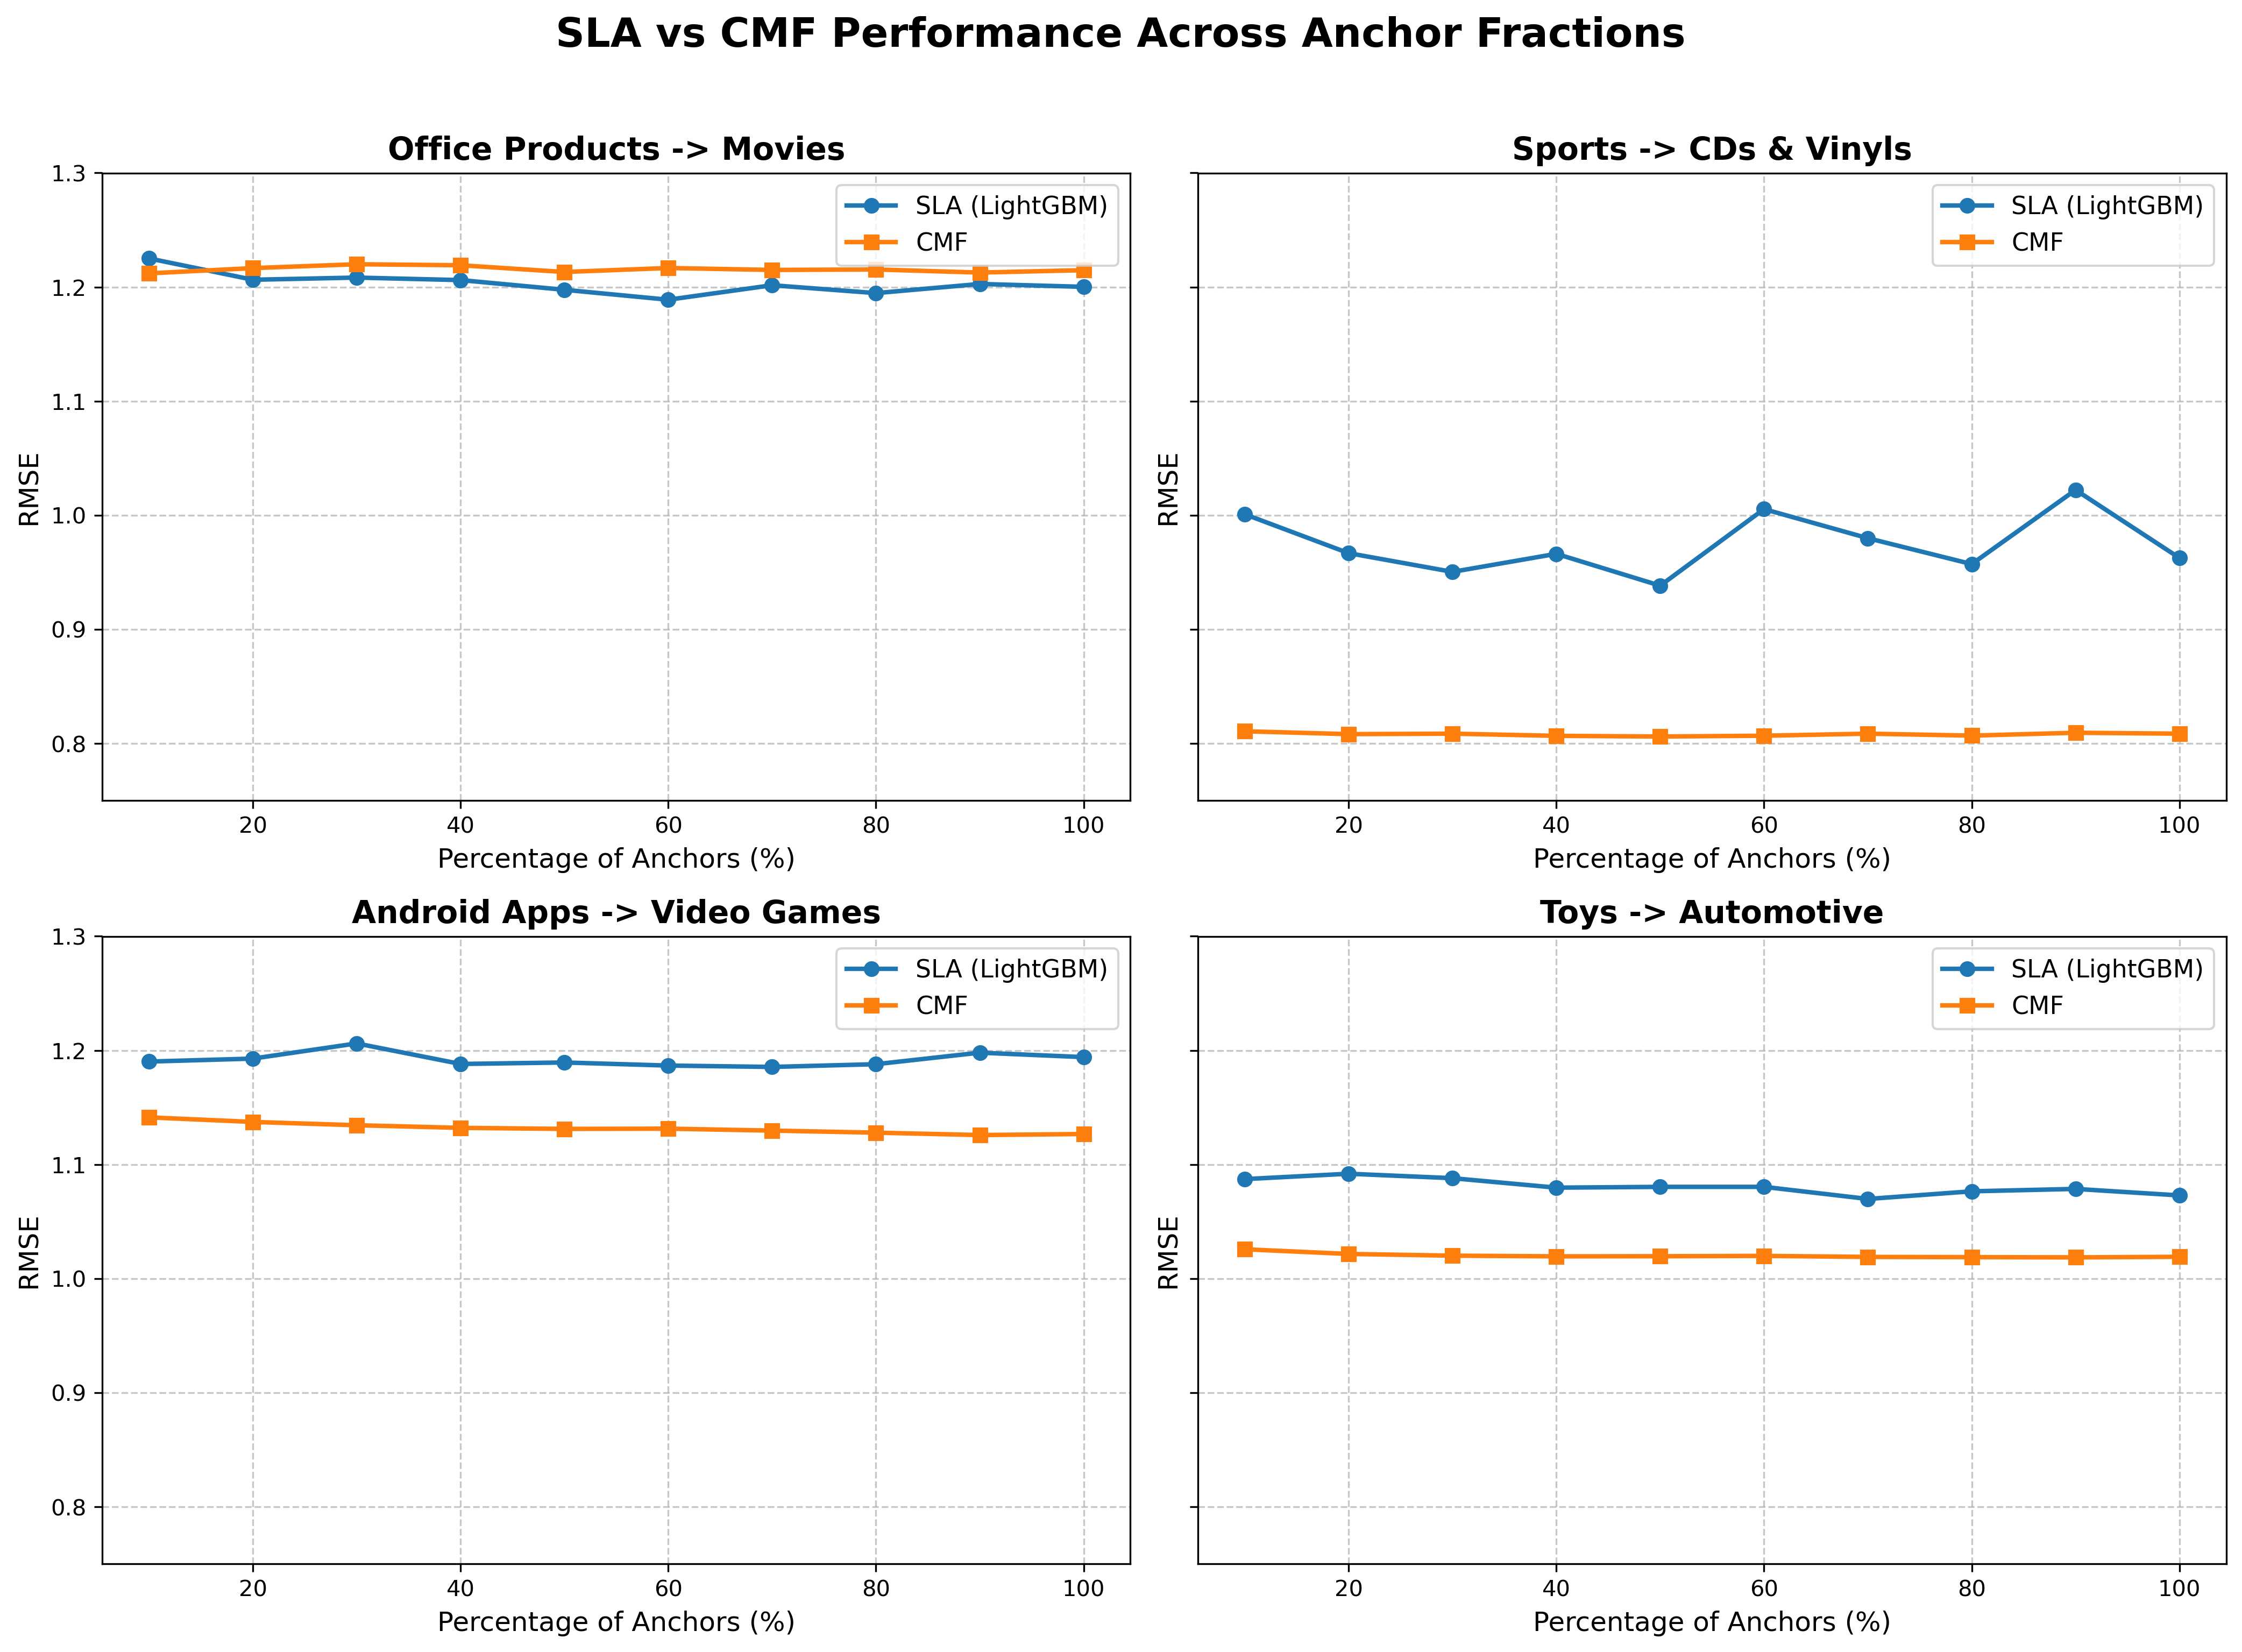
\includegraphics[width=\columnwidth]{combined_anchors_rmse.png}
    \caption{SLA vs CMF RMSE across anchor fractions. SLA maintains stable performance with few anchors.}
    \label{fig:anchors}
\end{figure}

\subsection{Training Time Comparison}

Table~\ref{tab:timing} compares end-to-end training times. SLA's runtime is dominated by the SVD computation and scales with matrix dimensions rather than the number of ratings, making it more predictable.

\begin{table}[h]
\centering
\caption{Training Time (50 epochs for CMF)}
\label{tab:timing}
\begin{tabular}{lcc}
\toprule
\textbf{Dataset Pair} & \textbf{SLA} & \textbf{CMF} \\
\midrule
Office$\to$Movies (193k ratings) & 46.2s & 88.1s \\
Sports$\to$CDs (132k ratings) & 46.5s & 64.9s \\
Apps$\to$Games (42k ratings) & 14.1s & 13.7s \\
Toys$\to$Auto (40k ratings) & 29.4s & 15.4s \\
\bottomrule
\end{tabular}
\end{table}

For the two largest datasets, SLA is 1.4--1.9$\times$ faster than CMF. On smaller datasets, the two methods are comparable.

\begin{figure}[h]
    \centering
    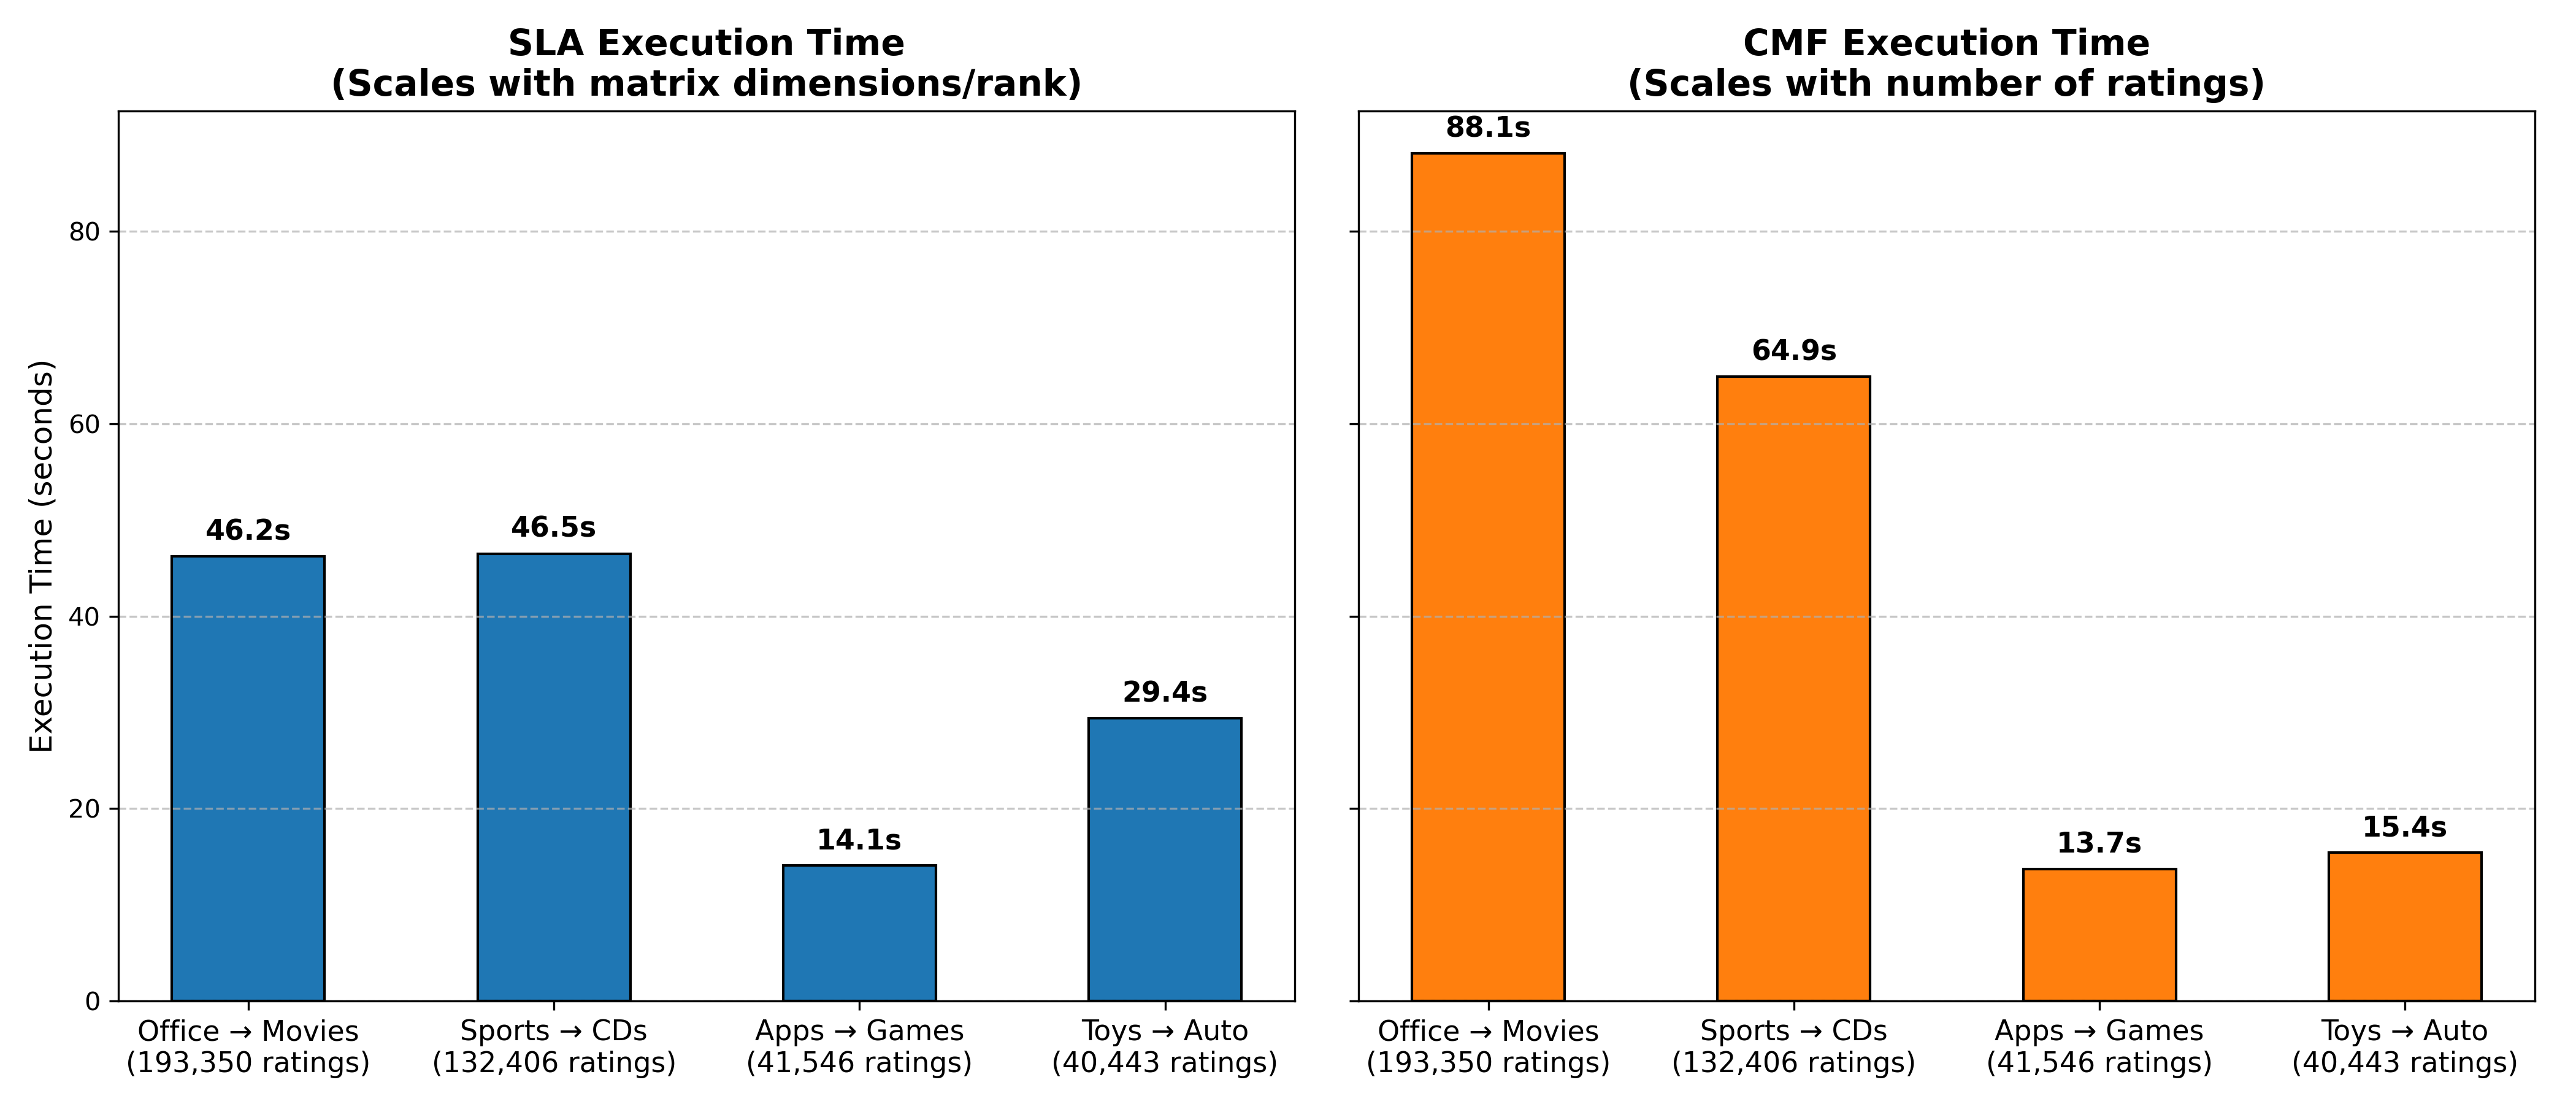
\includegraphics[width=\columnwidth]{timing_vs_density.png}
    \caption{SLA execution time scales with matrix dimensions/rank; CMF scales with number of ratings.}
    \label{fig:timing}
\end{figure}

\section{Discussion}

Our results reveal an important distinction between \emph{alignment quality} and \emph{prediction quality}. CMF achieves lower absolute RMSE because it jointly optimizes rating prediction across both domains, effectively learning a strong predictor. However, CMF's large alignment gap (up to 0.358 on Apps$\to$Games) indicates that its cross-domain transfer mechanism is relatively crude---the shared user embedding is a compromise between fitting source and target ratings rather than a principled structural alignment.

SLA, by contrast, achieves nearly lossless structural transfer (gaps as low as 0.012) because the Procrustes alignment directly minimizes structural mismatch. The theoretical bound confirms this: the alignment quality depends on the spectral gap $\gamma$ and anchor quality $\sigma_{\min}(X^TX)$, not on rating prediction accuracy.

This makes SLA most valuable as a \emph{transformation component} that can be composed with stronger predictors. The hybrid SLA-CMF results validate this: by injecting SLA's structural alignment into CMF's training pipeline, we obtain a model that benefits from both.

\section{Conclusion}

We have investigated Spectral Latent Alignment as a transformation technique for cross-domain recommendation. Our experiments demonstrate that SLA achieves alignment gaps 2.7--25$\times$ smaller than CMF across four Amazon dataset pairs, establishing it as a superior method for structural knowledge transfer. The method is theoretically grounded, with an excess-risk bound that decomposes into interpretable, empirically estimable terms. SLA's embeddings can warm-start CMF, yielding improvements on 3 of 4 dataset pairs.

Future work includes: (i) extending SLA to non-overlapping user settings using content-based anchors, (ii) combining SLA with modern GNN-based recommenders such as LightGCN~\cite{he2020}, and (iii) scaling to industrial datasets with millions of users.

\begin{thebibliography}{99}

\bibitem{cantador2015}
I.~Cantador, I.~Fern{\'a}ndez-Tob{\'\i}as, S.~Berkovsky, and P.~Cremonesi, ``Cross-domain recommender systems,'' in \emph{Recommender Systems Handbook}, Springer, 2015, pp.~919--959.

\bibitem{singh2008}
A.~P.~Singh and G.~J.~Gordon, ``Relational learning via collective matrix factorization,'' in \emph{Proc.\ 14th ACM SIGKDD Int.\ Conf.\ Knowledge Discovery and Data Mining}, 2008, pp.~650--658.

\bibitem{yuan2019}
F.~Yuan, L.~Yao, and B.~Benatallah, ``DARec: Deep domain adaptation for cross-domain recommendation via transferring rating patterns,'' in \emph{Proc.\ 28th Int.\ Joint Conf.\ Artificial Intelligence (IJCAI)}, 2019, pp.~4227--4233.

\bibitem{man2017}
T.~Man, H.~Shen, X.~Jin, and X.~Cheng, ``Cross-domain recommendation: An embedding and mapping approach,'' in \emph{Proc.\ 26th Int.\ Joint Conf.\ Artificial Intelligence (IJCAI)}, 2017, pp.~2464--2470.

\bibitem{hu2018}
G.~Hu, Y.~Zhang, and Q.~Yang, ``CoNet: Collaborative cross networks for cross-domain recommendation,'' in \emph{Proc.\ 27th ACM Int.\ Conf.\ Information and Knowledge Management (CIKM)}, 2018, pp.~667--676.

\bibitem{zhu2021}
F.~Zhu, Y.~Wang, C.~Chen, J.~Zhou, L.~Li, and G.~Liu, ``Cross-domain recommendation: Challenges, progress, and prospects,'' in \emph{Proc.\ 30th Int.\ Joint Conf.\ Artificial Intelligence (IJCAI)}, 2021, pp.~4721--4728.

\bibitem{khan2017}
M.~M.~Khan, R.~Ibrahim, and I.~Ghani, ``Cross domain recommender systems: A systematic literature review,'' \emph{ACM Computing Surveys}, vol.~50, no.~3, pp.~1--34, 2017.

\bibitem{li2009}
B.~Li, Q.~Yang, and X.~Xue, ``Can movies and books collaborate? Cross-domain collaborative filtering for sparsity reduction,'' in \emph{Proc.\ 21st Int.\ Joint Conf.\ Artificial Intelligence (IJCAI)}, 2009, pp.~2052--2057.

\bibitem{hu2013}
R.~Hu, L.~Nie, and X.~Wu, ``Personalized recommendation via cross-domain triadic factorization,'' in \emph{Proc.\ 22nd Int.\ World Wide Web Conf.\ (WWW)}, 2013, pp.~595--606.

\bibitem{elkahky2015}
A.~M.~Elkahky, Y.~Song, and X.~He, ``A multi-view deep learning approach for cross domain user modeling in recommendation systems,'' in \emph{Proc.\ 24th Int.\ World Wide Web Conf.\ (WWW)}, 2015, pp.~278--288.

\bibitem{cao2022}
J.~Cao, J.~Sheng, X.~Cong, T.~Liu, and B.~Wang, ``Cross-domain recommendation to cold-start users via variational information bottleneck,'' in \emph{Proc.\ IEEE Int.\ Conf.\ Data Engineering (ICDE)}, 2022, pp.~2209--2222.

\bibitem{ganin2016}
Y.~Ganin, E.~Ustinova, H.~Ajakan, P.~Germain, H.~Larochelle, F.~Laviolette, M.~Marchand, and V.~Lempitsky, ``Domain-adversarial training of neural networks,'' \emph{J.\ Machine Learning Research}, vol.~17, no.~59, pp.~1--35, 2016.

\bibitem{liu2017}
F.~Liu, R.~Tang, X.~He, F.~Zhang, M.~Zhang, and S.~Ma, ``Cross-domain recommendation via collaborative deep learning,'' in \emph{Proc.\ ACM SIGKDD Int.\ Conf.\ Knowledge Discovery and Data Mining}, 2017.

\bibitem{ying2018}
R.~Ying, R.~He, K.~Chen, P.~Eksombatchai, W.~L.~Hamilton, and J.~Leskovec, ``Graph convolutional neural networks for web-scale recommender systems,'' in \emph{Proc.\ 24th ACM SIGKDD Int.\ Conf.\ Knowledge Discovery and Data Mining}, 2018, pp.~974--983.

\bibitem{he2020}
X.~He, K.~Deng, X.~Wang, Y.~Li, Y.~Zhang, and M.~Wang, ``LightGCN: Simplifying and powering graph convolution network for recommendation,'' in \emph{Proc.\ 43rd Int.\ ACM SIGIR Conf.\ Research and Development in Information Retrieval}, 2020, pp.~639--648.

\bibitem{schoenemann1966}
P.~H.~Sch{\"o}nemann, ``A generalized solution of the orthogonal Procrustes problem,'' \emph{Psychometrika}, vol.~31, no.~1, pp.~1--10, 1966.

\bibitem{davis1970}
C.~Davis and W.~M.~Kahan, ``The rotation of eigenvectors by a perturbation.\ III,'' \emph{SIAM J.\ Numerical Analysis}, vol.~7, no.~1, pp.~1--46, 1970.

\bibitem{mcauley2015}
J.~McAuley, C.~Targett, Q.~Shi, and A.~van den Hengel, ``Image-based recommendations on styles and substitutes,'' in \emph{Proc.\ 38th Int.\ ACM SIGIR Conf.}, 2015, pp.~43--52.

\end{thebibliography}


\end{document}
